% Options for packages loaded elsewhere
\PassOptionsToPackage{unicode}{hyperref}
\PassOptionsToPackage{hyphens}{url}
%
\documentclass[
]{article}
\usepackage{amsmath,amssymb}
\usepackage{lmodern}
\usepackage{iftex}
\ifPDFTeX
  \usepackage[T1]{fontenc}
  \usepackage[utf8]{inputenc}
  \usepackage{textcomp} % provide euro and other symbols
\else % if luatex or xetex
  \usepackage{unicode-math}
  \defaultfontfeatures{Scale=MatchLowercase}
  \defaultfontfeatures[\rmfamily]{Ligatures=TeX,Scale=1}
\fi
% Use upquote if available, for straight quotes in verbatim environments
\IfFileExists{upquote.sty}{\usepackage{upquote}}{}
\IfFileExists{microtype.sty}{% use microtype if available
  \usepackage[]{microtype}
  \UseMicrotypeSet[protrusion]{basicmath} % disable protrusion for tt fonts
}{}
\makeatletter
\@ifundefined{KOMAClassName}{% if non-KOMA class
  \IfFileExists{parskip.sty}{%
    \usepackage{parskip}
  }{% else
    \setlength{\parindent}{0pt}
    \setlength{\parskip}{6pt plus 2pt minus 1pt}}
}{% if KOMA class
  \KOMAoptions{parskip=half}}
\makeatother
\usepackage{xcolor}
\IfFileExists{xurl.sty}{\usepackage{xurl}}{} % add URL line breaks if available
\IfFileExists{bookmark.sty}{\usepackage{bookmark}}{\usepackage{hyperref}}
\hypersetup{
  pdftitle={Risk outline - Reproducible Version},
  hidelinks,
  pdfcreator={LaTeX via pandoc}}
\urlstyle{same} % disable monospaced font for URLs
\usepackage[margin=1in]{geometry}
\usepackage{color}
\usepackage{fancyvrb}
\newcommand{\VerbBar}{|}
\newcommand{\VERB}{\Verb[commandchars=\\\{\}]}
\DefineVerbatimEnvironment{Highlighting}{Verbatim}{commandchars=\\\{\}}
% Add ',fontsize=\small' for more characters per line
\usepackage{framed}
\definecolor{shadecolor}{RGB}{248,248,248}
\newenvironment{Shaded}{\begin{snugshade}}{\end{snugshade}}
\newcommand{\AlertTok}[1]{\textcolor[rgb]{0.94,0.16,0.16}{#1}}
\newcommand{\AnnotationTok}[1]{\textcolor[rgb]{0.56,0.35,0.01}{\textbf{\textit{#1}}}}
\newcommand{\AttributeTok}[1]{\textcolor[rgb]{0.77,0.63,0.00}{#1}}
\newcommand{\BaseNTok}[1]{\textcolor[rgb]{0.00,0.00,0.81}{#1}}
\newcommand{\BuiltInTok}[1]{#1}
\newcommand{\CharTok}[1]{\textcolor[rgb]{0.31,0.60,0.02}{#1}}
\newcommand{\CommentTok}[1]{\textcolor[rgb]{0.56,0.35,0.01}{\textit{#1}}}
\newcommand{\CommentVarTok}[1]{\textcolor[rgb]{0.56,0.35,0.01}{\textbf{\textit{#1}}}}
\newcommand{\ConstantTok}[1]{\textcolor[rgb]{0.00,0.00,0.00}{#1}}
\newcommand{\ControlFlowTok}[1]{\textcolor[rgb]{0.13,0.29,0.53}{\textbf{#1}}}
\newcommand{\DataTypeTok}[1]{\textcolor[rgb]{0.13,0.29,0.53}{#1}}
\newcommand{\DecValTok}[1]{\textcolor[rgb]{0.00,0.00,0.81}{#1}}
\newcommand{\DocumentationTok}[1]{\textcolor[rgb]{0.56,0.35,0.01}{\textbf{\textit{#1}}}}
\newcommand{\ErrorTok}[1]{\textcolor[rgb]{0.64,0.00,0.00}{\textbf{#1}}}
\newcommand{\ExtensionTok}[1]{#1}
\newcommand{\FloatTok}[1]{\textcolor[rgb]{0.00,0.00,0.81}{#1}}
\newcommand{\FunctionTok}[1]{\textcolor[rgb]{0.00,0.00,0.00}{#1}}
\newcommand{\ImportTok}[1]{#1}
\newcommand{\InformationTok}[1]{\textcolor[rgb]{0.56,0.35,0.01}{\textbf{\textit{#1}}}}
\newcommand{\KeywordTok}[1]{\textcolor[rgb]{0.13,0.29,0.53}{\textbf{#1}}}
\newcommand{\NormalTok}[1]{#1}
\newcommand{\OperatorTok}[1]{\textcolor[rgb]{0.81,0.36,0.00}{\textbf{#1}}}
\newcommand{\OtherTok}[1]{\textcolor[rgb]{0.56,0.35,0.01}{#1}}
\newcommand{\PreprocessorTok}[1]{\textcolor[rgb]{0.56,0.35,0.01}{\textit{#1}}}
\newcommand{\RegionMarkerTok}[1]{#1}
\newcommand{\SpecialCharTok}[1]{\textcolor[rgb]{0.00,0.00,0.00}{#1}}
\newcommand{\SpecialStringTok}[1]{\textcolor[rgb]{0.31,0.60,0.02}{#1}}
\newcommand{\StringTok}[1]{\textcolor[rgb]{0.31,0.60,0.02}{#1}}
\newcommand{\VariableTok}[1]{\textcolor[rgb]{0.00,0.00,0.00}{#1}}
\newcommand{\VerbatimStringTok}[1]{\textcolor[rgb]{0.31,0.60,0.02}{#1}}
\newcommand{\WarningTok}[1]{\textcolor[rgb]{0.56,0.35,0.01}{\textbf{\textit{#1}}}}
\usepackage{graphicx}
\makeatletter
\def\maxwidth{\ifdim\Gin@nat@width>\linewidth\linewidth\else\Gin@nat@width\fi}
\def\maxheight{\ifdim\Gin@nat@height>\textheight\textheight\else\Gin@nat@height\fi}
\makeatother
% Scale images if necessary, so that they will not overflow the page
% margins by default, and it is still possible to overwrite the defaults
% using explicit options in \includegraphics[width, height, ...]{}
\setkeys{Gin}{width=\maxwidth,height=\maxheight,keepaspectratio}
% Set default figure placement to htbp
\makeatletter
\def\fps@figure{htbp}
\makeatother
\setlength{\emergencystretch}{3em} % prevent overfull lines
\providecommand{\tightlist}{%
  \setlength{\itemsep}{0pt}\setlength{\parskip}{0pt}}
\setcounter{secnumdepth}{-\maxdimen} % remove section numbering
\usepackage{booktabs}
\usepackage{longtable}
\usepackage{array}
\usepackage{multirow}
\usepackage{wrapfig}
\usepackage{float}
\usepackage{colortbl}
\usepackage{pdflscape}
\usepackage{tabu}
\usepackage{threeparttable}
\usepackage{threeparttablex}
\usepackage[normalem]{ulem}
\usepackage{makecell}
\usepackage{xcolor}
\ifLuaTeX
  \usepackage{selnolig}  % disable illegal ligatures
\fi

\title{Risk outline - Reproducible Version}
\author{}
\date{\vspace{-2.5em}}

\begin{document}
\maketitle

\hypertarget{survey-data-overview}{%
\subsubsection{Survey data overview}\label{survey-data-overview}}

\textbf{Job risk model}

We use Pulse data from phase 3.1, 3.2, and 3.3. The data for these
phases pertain to data collected across the following periods:

\begin{itemize}
\tightlist
\item
  Phase 3.1: April 14, 2021 -- July 5, 2021
\item
  Phase 3.2: July 21, 2021 -- October 11, 2021
\item
  Phase 3.3: December 1, 2021 -- February 7, 2022
\item
  Phase 3.4: March 2, 2022 - May 9, 2022
\end{itemize}

Pulse surveys prior to phase 3.1 do not contain the question about the
job setting of respondents that allows us to categorize employees.

\textbf{Omicron concerns + impetus for creating risk of infection by
specific severity levels}

The period starting from mid-Phase 3.3 and continuing for phase 3.4
contains data collected during a time of high prevalence of the Omicron
variant. Using CDC data on variant proportions, we see that beginning
with the week ending on December 27, 2021, the Omicron variant
constituted over half of all COVID infections of the US.

\begin{Shaded}
\begin{Highlighting}[]
\FunctionTok{read.csv}\NormalTok{(}\StringTok{"data\_files/covid/covid\_variant\_proportions.csv"}\NormalTok{) }\SpecialCharTok{\%\textgreater{}\%}
  \FunctionTok{filter}\NormalTok{(modeltype }\SpecialCharTok{==} \StringTok{"smoothed"}\NormalTok{) }\SpecialCharTok{\%\textgreater{}\%}
  \FunctionTok{group\_by}\NormalTok{(week\_ending,variant) }\SpecialCharTok{\%\textgreater{}\%}
  \FunctionTok{arrange}\NormalTok{(}\FunctionTok{desc}\NormalTok{(published\_date)) }\SpecialCharTok{\%\textgreater{}\%}
  \FunctionTok{slice}\NormalTok{(}\DecValTok{1}\SpecialCharTok{:}\DecValTok{1}\NormalTok{) }\SpecialCharTok{\%\textgreater{}\%}
  \FunctionTok{mutate}\NormalTok{(}\AttributeTok{week\_ending =} \FunctionTok{as.Date}\NormalTok{(}\FunctionTok{substr}\NormalTok{(week\_ending,}\DecValTok{1}\NormalTok{,}\DecValTok{10}\NormalTok{),}\AttributeTok{format=}\StringTok{"\%m/\%d/\%Y"}\NormalTok{),}
         \AttributeTok{published\_date =} \FunctionTok{as.Date}\NormalTok{(}\FunctionTok{substr}\NormalTok{(published\_date,}\DecValTok{1}\NormalTok{,}\DecValTok{10}\NormalTok{),}\AttributeTok{format=}\StringTok{"\%m/\%d/\%Y"}\NormalTok{),}
         \AttributeTok{variant =} \FunctionTok{case\_when}\NormalTok{(}
\NormalTok{           variant }\SpecialCharTok{==} \StringTok{"BA.1.1"} \SpecialCharTok{\textasciitilde{}} \StringTok{"Omicron"}\NormalTok{,}
\NormalTok{           variant }\SpecialCharTok{==} \StringTok{"BA.2"} \SpecialCharTok{\textasciitilde{}} \StringTok{"Omicron"}\NormalTok{,}
\NormalTok{           variant }\SpecialCharTok{==} \StringTok{"B.1.1.529"} \SpecialCharTok{\textasciitilde{}} \StringTok{"Omicron"}\NormalTok{,}
\NormalTok{           variant }\SpecialCharTok{==} \StringTok{"BA.2.12.1"} \SpecialCharTok{\textasciitilde{}} \StringTok{"Omicron"}\NormalTok{,}
\NormalTok{           variant }\SpecialCharTok{==} \StringTok{"B.1.1.7"} \SpecialCharTok{\textasciitilde{}} \StringTok{"Alpha"}\NormalTok{,}
\NormalTok{           variant }\SpecialCharTok{==} \StringTok{"AY.1"} \SpecialCharTok{\textasciitilde{}} \StringTok{"Delta"}\NormalTok{,}
\NormalTok{           variant }\SpecialCharTok{==} \StringTok{"AY.2"} \SpecialCharTok{\textasciitilde{}} \StringTok{"Delta"}\NormalTok{,}
\NormalTok{           variant }\SpecialCharTok{==} \StringTok{"B.1.617.2"} \SpecialCharTok{\textasciitilde{}} \StringTok{"Delta"}\NormalTok{,}
\NormalTok{           variant }\SpecialCharTok{==} \StringTok{"Other"} \SpecialCharTok{\textasciitilde{}} \StringTok{"Other"}\NormalTok{)) }\SpecialCharTok{\%\textgreater{}\%}
  \FunctionTok{ggplot}\NormalTok{(}\FunctionTok{aes}\NormalTok{(}\AttributeTok{x=}\FunctionTok{as.Date}\NormalTok{(week\_ending),}\AttributeTok{y=}\NormalTok{share,}\AttributeTok{fill=}\NormalTok{variant,}\AttributeTok{col=}\NormalTok{variant)) }\SpecialCharTok{+} 
  \FunctionTok{geom\_col}\NormalTok{() }\SpecialCharTok{+}
  \FunctionTok{scale\_x\_date}\NormalTok{(}\AttributeTok{date\_breaks =} \StringTok{"weeks"}\NormalTok{) }\SpecialCharTok{+}
  \FunctionTok{theme\_minimal}\NormalTok{() }\SpecialCharTok{+} 
  \FunctionTok{theme}\NormalTok{(}\AttributeTok{axis.text.x =} \FunctionTok{element\_text}\NormalTok{(}\AttributeTok{angle =} \DecValTok{90}\NormalTok{, }\AttributeTok{vjust =} \FloatTok{0.5}\NormalTok{, }\AttributeTok{hjust=}\DecValTok{1}\NormalTok{)) }\SpecialCharTok{+}
  \FunctionTok{theme}\NormalTok{(}\AttributeTok{text =} \FunctionTok{element\_text}\NormalTok{(}\AttributeTok{family =} \StringTok{"Georgia"}\NormalTok{,}\AttributeTok{size=}\DecValTok{9}\NormalTok{)) }\SpecialCharTok{+}
  \FunctionTok{geom\_hline}\NormalTok{(}\AttributeTok{yintercept=}\FloatTok{0.5}\NormalTok{) }\SpecialCharTok{+} 
  \FunctionTok{labs}\NormalTok{(}\AttributeTok{x =} \StringTok{"Date"}\NormalTok{,}\AttributeTok{y =} \StringTok{"Share Infections"}\NormalTok{,}\AttributeTok{title =} \StringTok{"Variant Proportions"}\NormalTok{)}
\end{Highlighting}
\end{Shaded}

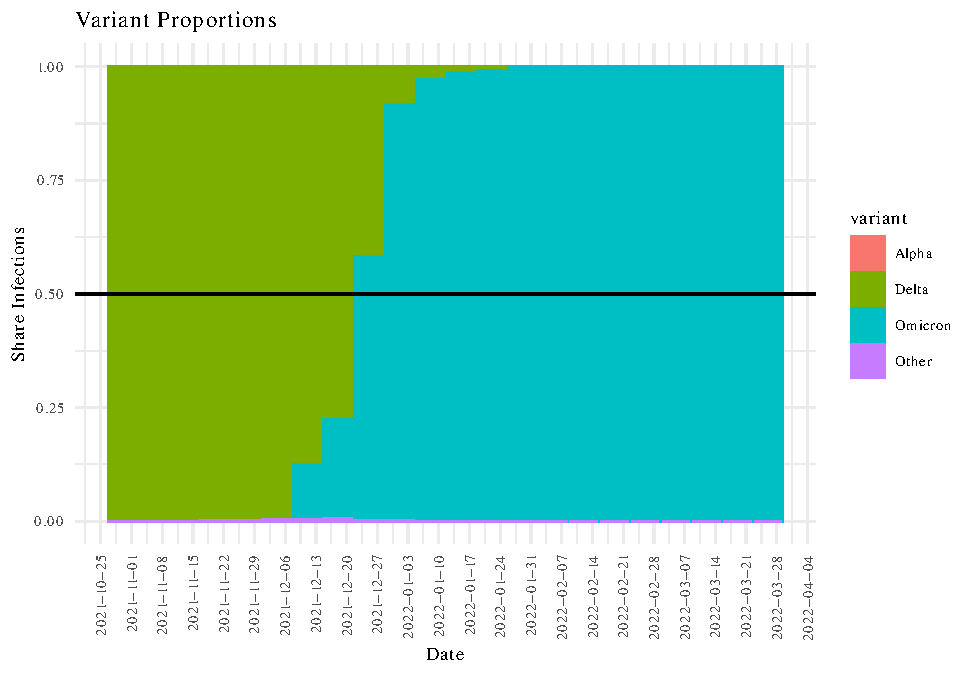
\includegraphics{risk_of_infection_files/figure-latex/unnamed-chunk-2-1.pdf}

Because of the highly contagious nature of the variant, we worried
readers might think that merely getting infected isn't a big deal given
the high share of adults infected at least once. We are also interested
in measuring the absolute amount of noxiousness and how it compares to
the pre-pandemic period, which means we need a risk measure that is
comparable to the types of workplace risk that existed prior to the
pandemic. It makes sense to think of an injury ending in death in the
same way we think about a covid infection ending in death, but comparing
a non-fatal injury such as a cut or laceration with a mild case of
covid, or a bad fracture with a case of long covid, is less
straightforward. We resolve this apples-to-apples issue by converting
the risk of a covid infection to the risk of a mild to moderate
infection or a covid hospitalization. We also calculate the risk for the
infection to result in a case of long covid. For each type of infection
severity, we can give an estimate for the number of days away from work
resulting from it by using data on the average recovery time for each
type. Finally, we use BLS data collected prior to the pandemic that
records the total number of injuries recorded in each industry and the
respective recovery times. The bottomline: if a covid infection
contracted on the job took 15 days to recover from, we argue the
severity of the infection is comparable to a workplace injury that
resulted in the worker taking 15 days away from the job.

\hypertarget{creating-job-categories}{%
\subsubsection{Creating job categories}\label{creating-job-categories}}

We start by assigning a job category to each respondent. We create job
categories by combining the type of work the respondent does and their
education level. An important point: we only keep respondents who were
18 or older at the time of being surveyed.

\begin{enumerate}
\def\labelenumi{\arabic{enumi}.}
\tightlist
\item
  Work in the last 7 days

  \begin{itemize}
  \tightlist
  \item
    Variable name: any\_work
  \item
    Phase 3.1, 3.2, 3.3 and 3.4: ``In the last 7 days, have you done any
    work for pay or profit?''
  \end{itemize}
\item
  Work outside the home

  \begin{itemize}
  \tightlist
  \item
    Variable name: work\_outside\_home
  \item
    Phase 3.1: ``Since January 1, 2021, have you worked or volunteered
    outside your home?''
  \item
    Phase 3.2, 3.3, and 3.4: ``In the last 7 days, have you worked or
    volunteered outside your home?''
  \end{itemize}
\item
  Setting of work outside home

  \begin{itemize}
  \tightlist
  \item
    Variable name: setting
  \item
    Phase 3.1: ``Since January 1, 2021, which best describes the primary
    location/setting where you worked or volunteered outside your
    home?''
  \item
    Phase 3.2, 3.3, and 3.4: ``In the last 7 days, which best describes
    the primary location/setting where you worked or volunteered outside
    your home?''
  \end{itemize}
\item
  Reason not work for pay or profit

  \begin{itemize}
  \tightlist
  \item
    Variable name: reason\_not\_work
  \item
    Phase 3.1, 3.2, 3.3, and 3.4: ``What is your main reason for not
    working for pay or profit?''
  \end{itemize}
\end{enumerate}

\textbf{Categorization}

\begin{itemize}
\tightlist
\item
  In-person workers

  \begin{itemize}
  \tightlist
  \item
    Has worked in the last 7 days (any\_work = 1)
  \item
    Worked or volunteered outside the home (work\_outside\_home = 1)
  \end{itemize}
\item
  Remote workers

  \begin{itemize}
  \tightlist
  \item
    Has worked in the last 7 days (any\_work = 1)
  \item
    Has not worked or volunteered outside the home (work\_outside\_home
    = 2)
  \end{itemize}
\item
  Unemployed

  \begin{itemize}
  \tightlist
  \item
    Has not worked in the last 7 days (any\_work = 2)
  \item
    Main reason for not working for pay or profit:

    \begin{itemize}
    \tightlist
    \item
      Was concerned about getting or spreading the coronavirus
      (reason\_not\_work = 5)
    \item
      Was laid off or furloughed due to coronavirus pandemic
      (reason\_not\_work = 8)
    \item
      Employer closed temporarily due to coronavirus pandemic
      (reason\_not\_work = 9)
    \item
      Employer went out of business due to coronavirus pandemic
      (reason\_not\_work = 10)
    \item
      I do/did not have transportation to work (reason\_not\_work = 11)
    \end{itemize}
  \end{itemize}
\item
  NILF

  \begin{itemize}
  \tightlist
  \item
    Has not worked in the last 7 days (any\_work = 2)
  \item
    Main reason for not working for pay or profit:

    \begin{itemize}
    \tightlist
    \item
      I did not want to be employed at this time (reason\_not\_work = 1)
    \item
      I am/was sick with coronavirus symptoms or caring for someone who
      was sick with coronavirus symptoms (reason\_not\_work = 2)
    \item
      I am/was caring for children not in school or daycare
      (reason\_not\_work = 3)
    \item
      I am/was caring for an elderly person (reason\_not\_work = 4)
    \item
      I am/was sick (not coronavirus related) or disabled
      (reason\_not\_work = 6)
    \item
      I am retired (reason\_not\_work = 7)
    \item
      Other reason, please specify (reason\_not\_work = 12)
    \end{itemize}
  \end{itemize}
\end{itemize}

\textbf{Education Levels} We create 4 education categories:

\begin{enumerate}
\def\labelenumi{\arabic{enumi}.}
\tightlist
\item
  Less than high school graduate
\item
  High school graduate or GED
\item
  Some college or associate's degree
\item
  Bachelor's degree or higher
\end{enumerate}

\textbf{Combining education and setting data}

For the categories, ``Working from home'', ``Unemployed'', and ``NILF'',
we collapse across all 4 education categories as the type of work and
riskiness of it should not vary in these categories. Due to the
relatively small size of some of these job categories, we also make the
following changes to our job categories:

\begin{enumerate}
\def\labelenumi{\arabic{enumi}.}
\tightlist
\item
  Combine the ``less than high school'' and ``high school'' categories
  for ``correctional facilities''.
\item
  Combine the 4 ``health care'' and 4 ``death care'' categories into 4
  ``health and death care'' categories.
\item
  Combine the ``less than high school'' and ``high school'' categories
  for public transit.
\item
  Combine the ``less than high school'' and ``high school'' categories
  for USPS.
\end{enumerate}

We arrive at a final list of 60 job categories.

\begin{figure}
\centering
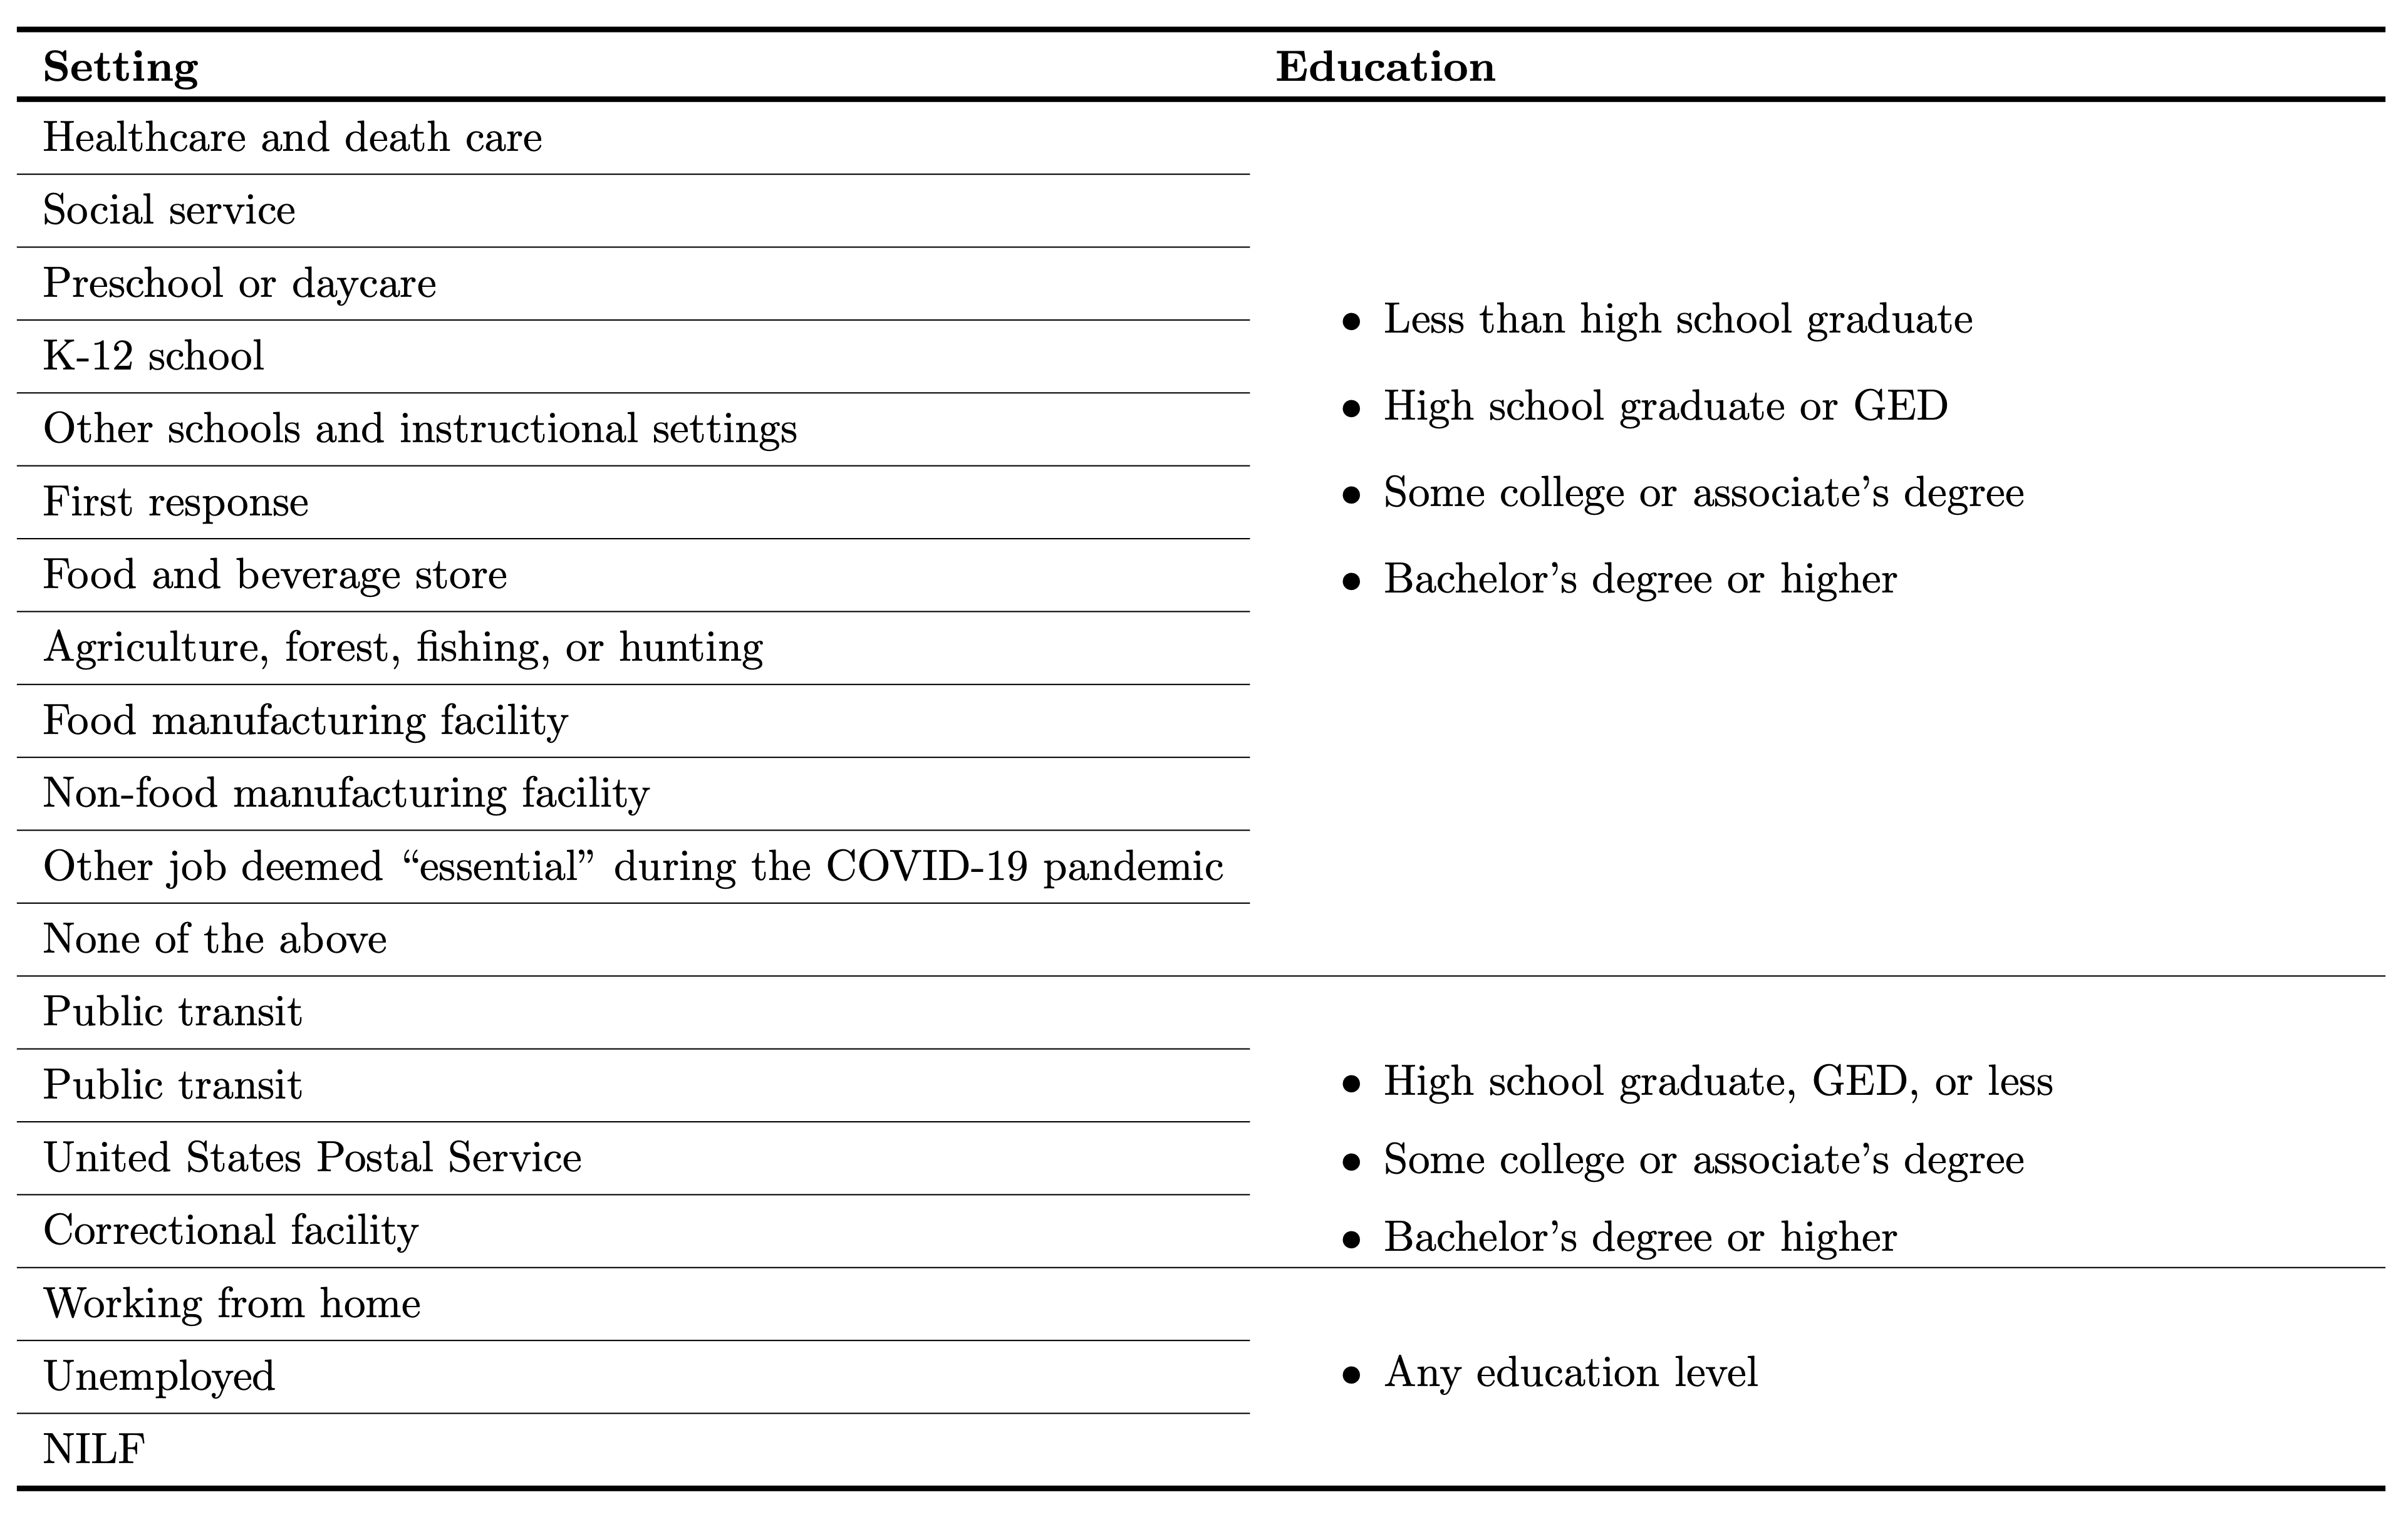
\includegraphics{"figures/job_categories.png"}
\caption{Job categories}
\end{figure}

Loading Pulse data, selecting relevant variables, renaming, and
cleaning:

\begin{Shaded}
\begin{Highlighting}[]
\NormalTok{clean\_vars }\OtherTok{\textless{}{-}} \FunctionTok{read.csv}\NormalTok{(}\StringTok{"data\_files/cleanvariables/pulse\_cleanvars.csv"}\NormalTok{)}
\NormalTok{recode\_vars }\OtherTok{\textless{}{-}} \FunctionTok{read.csv}\NormalTok{(}\StringTok{"data\_files/cleanvariables/pulse\_recode.csv"}\NormalTok{)}
\NormalTok{set\_educ\_to\_job }\OtherTok{\textless{}{-}} \FunctionTok{read.csv}\NormalTok{(}\StringTok{"data\_files/cleanvariables/pulse\_setting\_education\_to\_job.csv"}\NormalTok{) }\SpecialCharTok{\%\textgreater{}\%} \FunctionTok{mutate}\NormalTok{(}\AttributeTok{setting =} \FunctionTok{tolower}\NormalTok{(setting))}
\end{Highlighting}
\end{Shaded}

\begin{Shaded}
\begin{Highlighting}[]
\NormalTok{open }\OtherTok{\textless{}{-}} \ControlFlowTok{function}\NormalTok{(phase)\{}
\NormalTok{  filepath }\OtherTok{=} \FunctionTok{paste0}\NormalTok{(}\StringTok{"data\_files/pulse/phase"}\NormalTok{,}\FunctionTok{as.character}\NormalTok{(phase),}\StringTok{"/"}\NormalTok{)}
\NormalTok{  df }\OtherTok{\textless{}{-}} \FunctionTok{list.files}\NormalTok{(}\AttributeTok{path =}\NormalTok{ filepath,}
           \AttributeTok{pattern =} \StringTok{"*.csv"}\NormalTok{,}
           \AttributeTok{full.names =}\NormalTok{ T) }\SpecialCharTok{\%\textgreater{}\%} 
    \FunctionTok{map\_df}\NormalTok{(}\SpecialCharTok{\textasciitilde{}}\FunctionTok{read\_csv}\NormalTok{(.)) }\SpecialCharTok{\%\textgreater{}\%} 
\NormalTok{  dplyr}\SpecialCharTok{::}\FunctionTok{select}\NormalTok{(clean\_vars[clean\_vars}\SpecialCharTok{$}\NormalTok{phase }\SpecialCharTok{==}\NormalTok{ phase,]}\SpecialCharTok{$}\NormalTok{pulsename) }\SpecialCharTok{\%\textgreater{}\%} 
\NormalTok{  purrr}\SpecialCharTok{::}\FunctionTok{set\_names}\NormalTok{(clean\_vars[clean\_vars}\SpecialCharTok{$}\NormalTok{phase }\SpecialCharTok{==}\NormalTok{ phase,]}\SpecialCharTok{$}\NormalTok{newname)}
  \FunctionTok{return}\NormalTok{(df)}
\NormalTok{\}}
\end{Highlighting}
\end{Shaded}

\begin{Shaded}
\begin{Highlighting}[]
\NormalTok{recode }\OtherTok{\textless{}{-}} \ControlFlowTok{function}\NormalTok{(df,x,curr\_phase)\{}
\NormalTok{  df }\OtherTok{\textless{}{-}} \FunctionTok{merge}\NormalTok{(df,recode\_vars }\SpecialCharTok{\%\textgreater{}\%}
          \FunctionTok{filter}\NormalTok{(type }\SpecialCharTok{==}\NormalTok{ x }\SpecialCharTok{\&}\NormalTok{ phase }\SpecialCharTok{==}\NormalTok{ curr\_phase) }\SpecialCharTok{\%\textgreater{}\%}
          \FunctionTok{select}\NormalTok{(}\SpecialCharTok{{-}}\NormalTok{phase) }\SpecialCharTok{\%\textgreater{}\%}
\NormalTok{          dplyr}\SpecialCharTok{::}\FunctionTok{rename}\NormalTok{(\{\{x\}\} }\SpecialCharTok{:}\ErrorTok{=}\NormalTok{ oldvar))}
  \FunctionTok{return}\NormalTok{(df)}
\NormalTok{\}}
\end{Highlighting}
\end{Shaded}

Clean up data steps:

\begin{itemize}
\tightlist
\item
  Removed respondents born after 2003
\item
  Removed respondents missing responses necessary for categorization
\item
  Categorizing remote workers, nilf, and unemployed
\item
  Recoding variables from numbers to text
\end{itemize}

\begin{Shaded}
\begin{Highlighting}[]
\NormalTok{clean }\OtherTok{\textless{}{-}} \ControlFlowTok{function}\NormalTok{(df, phase)\{}
\NormalTok{ nilf }\OtherTok{\textless{}{-}} \FunctionTok{c}\NormalTok{(}\DecValTok{1}\NormalTok{,}\DecValTok{2}\NormalTok{,}\DecValTok{3}\NormalTok{,}\DecValTok{4}\NormalTok{,}\DecValTok{6}\NormalTok{,}\DecValTok{7}\NormalTok{,}\DecValTok{12}\NormalTok{)}
\NormalTok{ df }\OtherTok{\textless{}{-}}\NormalTok{ df }\SpecialCharTok{\%\textgreater{}\%} 
  \FunctionTok{filter}\NormalTok{(birth\_year }\SpecialCharTok{\textless{}=} \DecValTok{2003} \SpecialCharTok{\&}\NormalTok{ work\_outside\_home }\SpecialCharTok{\textgreater{}} \DecValTok{0} \SpecialCharTok{\&}\NormalTok{ setting }\SpecialCharTok{!=} \SpecialCharTok{{-}}\DecValTok{99} \SpecialCharTok{\&}\NormalTok{ reason\_not\_work }\SpecialCharTok{!=} \SpecialCharTok{{-}}\DecValTok{99}\NormalTok{) }\SpecialCharTok{\%\textgreater{}\%}
  \FunctionTok{mutate}\NormalTok{(}\AttributeTok{setting =} \FunctionTok{case\_when}\NormalTok{(}
\NormalTok{    work\_outside\_home }\SpecialCharTok{==} \DecValTok{2} \SpecialCharTok{\&}\NormalTok{ any\_work }\SpecialCharTok{==} \DecValTok{1} \SpecialCharTok{\textasciitilde{}} \DecValTok{20}\NormalTok{,}
\NormalTok{    any\_work }\SpecialCharTok{==} \DecValTok{2} \SpecialCharTok{\&} \SpecialCharTok{!}\NormalTok{(reason\_not\_work }\SpecialCharTok{\%in\%}\NormalTok{ nilf) }\SpecialCharTok{\textasciitilde{}} \DecValTok{21}\NormalTok{,}
\NormalTok{    any\_work }\SpecialCharTok{==} \DecValTok{2} \SpecialCharTok{\&}\NormalTok{ reason\_not\_work }\SpecialCharTok{\%in\%}\NormalTok{ nilf }\SpecialCharTok{\textasciitilde{}} \DecValTok{22}\NormalTok{,}
    \ConstantTok{TRUE} \SpecialCharTok{\textasciitilde{}}\NormalTok{ setting)) }\SpecialCharTok{\%\textgreater{}\%}
  \FunctionTok{filter}\NormalTok{(setting }\SpecialCharTok{\textgreater{}} \DecValTok{0}\NormalTok{) }\SpecialCharTok{\%\textgreater{}\%}
  \FunctionTok{mutate}\NormalTok{(}\AttributeTok{race\_ethnicity =} \FunctionTok{if\_else}\NormalTok{(hisp\_ethnicity }\SpecialCharTok{==} \DecValTok{2}\NormalTok{,}\DecValTok{5}\NormalTok{,race)) }\SpecialCharTok{\%\textgreater{}\%}
  \FunctionTok{left\_join}\NormalTok{(}\FunctionTok{unique}\NormalTok{(}\FunctionTok{get}\NormalTok{(}\FunctionTok{data}\NormalTok{(}\StringTok{"fips\_codes"}\NormalTok{)) }\SpecialCharTok{\%\textgreater{}\%} 
              \FunctionTok{select}\NormalTok{(state\_code,state\_name) }\SpecialCharTok{\%\textgreater{}\%} 
\NormalTok{              dplyr}\SpecialCharTok{::}\FunctionTok{rename}\NormalTok{(}\StringTok{"state"} \OtherTok{=} \StringTok{"state\_code"}\NormalTok{))) }\SpecialCharTok{\%\textgreater{}\%}
  \FunctionTok{select}\NormalTok{(}\SpecialCharTok{{-}}\NormalTok{state) }\SpecialCharTok{\%\textgreater{}\%} 
\NormalTok{  dplyr}\SpecialCharTok{::}\FunctionTok{rename}\NormalTok{(}\AttributeTok{state =}\NormalTok{ state\_name)}
 
 \ControlFlowTok{for}\NormalTok{(x }\ControlFlowTok{in} \FunctionTok{unique}\NormalTok{(recode\_vars}\SpecialCharTok{$}\NormalTok{type))\{}
\NormalTok{   df }\OtherTok{\textless{}{-}} \FunctionTok{recode}\NormalTok{(df,x,phase) }\SpecialCharTok{\%\textgreater{}\%} 
     \FunctionTok{select}\NormalTok{(}\SpecialCharTok{{-}}\NormalTok{type,}\SpecialCharTok{{-}}\NormalTok{\{\{x\}\}) }\SpecialCharTok{\%\textgreater{}\%}
\NormalTok{     dplyr}\SpecialCharTok{::}\FunctionTok{rename}\NormalTok{(\{\{x\}\} }\SpecialCharTok{:}\ErrorTok{=}\NormalTok{ newvar) }
\NormalTok{ \}}
 \FunctionTok{return}\NormalTok{(df)}
\NormalTok{\}}
\end{Highlighting}
\end{Shaded}

Combining setting information with education level to create job
categories.

\begin{Shaded}
\begin{Highlighting}[]
\NormalTok{make\_job }\OtherTok{\textless{}{-}} \ControlFlowTok{function}\NormalTok{(df)\{}
\NormalTok{  df }\OtherTok{\textless{}{-}} \FunctionTok{merge}\NormalTok{(df,set\_educ\_to\_job,}\AttributeTok{by=}\FunctionTok{c}\NormalTok{(}\StringTok{"setting"}\NormalTok{,}\StringTok{"education"}\NormalTok{))}
  \FunctionTok{return}\NormalTok{(df)}
\NormalTok{\}}
\end{Highlighting}
\end{Shaded}

\begin{Shaded}
\begin{Highlighting}[]
\NormalTok{process }\OtherTok{\textless{}{-}} \ControlFlowTok{function}\NormalTok{(phase)\{}
\NormalTok{  df }\OtherTok{\textless{}{-}} \FunctionTok{open}\NormalTok{(phase)}
\NormalTok{  df }\OtherTok{\textless{}{-}} \FunctionTok{clean}\NormalTok{(df,phase)}
\NormalTok{  df }\OtherTok{\textless{}{-}} \FunctionTok{make\_job}\NormalTok{(df)}
  \FunctionTok{return}\NormalTok{(df)}
\NormalTok{\}}
\end{Highlighting}
\end{Shaded}

Obtaining clean data files:

\begin{Shaded}
\begin{Highlighting}[]
\NormalTok{phase3}\FloatTok{.1} \OtherTok{\textless{}{-}} \FunctionTok{process}\NormalTok{(}\FloatTok{3.1}\NormalTok{)}
\NormalTok{phase3}\FloatTok{.2} \OtherTok{\textless{}{-}} \FunctionTok{process}\NormalTok{(}\FloatTok{3.2}\NormalTok{)}
\NormalTok{phase3}\FloatTok{.3} \OtherTok{\textless{}{-}} \FunctionTok{process}\NormalTok{(}\FloatTok{3.3}\NormalTok{)}
\NormalTok{phase3}\FloatTok{.4} \OtherTok{\textless{}{-}} \FunctionTok{process}\NormalTok{(}\FloatTok{3.4}\NormalTok{)}
\end{Highlighting}
\end{Shaded}

Exporting processed files:

\begin{Shaded}
\begin{Highlighting}[]
\FunctionTok{write.csv}\NormalTok{(phase3}\FloatTok{.1}\NormalTok{,}\StringTok{"data\_files/pulse/processed/phase3.1.csv"}\NormalTok{)}
\FunctionTok{write.csv}\NormalTok{(phase3}\FloatTok{.2}\NormalTok{,}\StringTok{"data\_files/pulse/processed/phase3.2.csv"}\NormalTok{)}
\FunctionTok{write.csv}\NormalTok{(phase3}\FloatTok{.3}\NormalTok{,}\StringTok{"data\_files/pulse/processed/phase3.3.csv"}\NormalTok{)}
\FunctionTok{write.csv}\NormalTok{(phase3}\FloatTok{.4}\NormalTok{,}\StringTok{"data\_files/pulse/processed/phase3.4.csv"}\NormalTok{)}
\end{Highlighting}
\end{Shaded}

\textbf{Sanity checking telework}

Doing a sanity check the latter phases, ``In the last 7 days, have you
or your household done any of the following\ldots{} Teleworked or worked
from home?'' we find that 34\% of our ``WFH'' employees said they didn't
work from home.

To handle these ``inconsistent'' responses, we treat it as missing
impute these settings by using a respondent's age, education level,
household income, etc. to predict the missing setting.

\begin{Shaded}
\begin{Highlighting}[]
\NormalTok{temp\_merge }\OtherTok{\textless{}{-}} \FunctionTok{rbind}\NormalTok{(phase3}\FloatTok{.2}\NormalTok{,phase3}\FloatTok{.3}\NormalTok{,phase3}\FloatTok{.4}\NormalTok{)}
\NormalTok{temp\_merge }\SpecialCharTok{\%\textgreater{}\%}
  \FunctionTok{filter}\NormalTok{(setting }\SpecialCharTok{==} \StringTok{"working from home"} \SpecialCharTok{\&}\NormalTok{ teleworked }\SpecialCharTok{\textgreater{}} \DecValTok{0}\NormalTok{) }\SpecialCharTok{\%\textgreater{}\%}
  \FunctionTok{mutate}\NormalTok{(}\AttributeTok{teleworked =} \FunctionTok{if\_else}\NormalTok{(teleworked }\SpecialCharTok{==} \DecValTok{1}\NormalTok{,}\StringTok{"Yes"}\NormalTok{,}\StringTok{"No"}\NormalTok{)) }\SpecialCharTok{\%\textgreater{}\%}
\NormalTok{  dplyr}\SpecialCharTok{::}\FunctionTok{group\_by}\NormalTok{(teleworked) }\SpecialCharTok{\%\textgreater{}\%}
\NormalTok{  dplyr}\SpecialCharTok{::}\FunctionTok{summarise}\NormalTok{(}\AttributeTok{count =} \FunctionTok{n}\NormalTok{()) }\SpecialCharTok{\%\textgreater{}\%}
  \FunctionTok{mutate}\NormalTok{(}\AttributeTok{percent\_teleworked =}\NormalTok{ count}\SpecialCharTok{/}\FunctionTok{sum}\NormalTok{(count)) }\SpecialCharTok{\%\textgreater{}\%}
  \FunctionTok{ggplot}\NormalTok{(}\FunctionTok{aes}\NormalTok{(}\AttributeTok{x=}\NormalTok{teleworked,}
             \AttributeTok{y=}\NormalTok{percent\_teleworked)) }\SpecialCharTok{+} 
  \FunctionTok{theme\_minimal}\NormalTok{() }\SpecialCharTok{+} 
  \FunctionTok{labs}\NormalTok{(}\AttributeTok{x=}\StringTok{"In the last 7 days, have you or your household teleworked?"}\NormalTok{,}
       \AttributeTok{y=}\StringTok{"\% of work from home respondents"}\NormalTok{,}
       \AttributeTok{title =} \StringTok{"Inconsisent categorization"}\NormalTok{,}
       \AttributeTok{subtitle =} \StringTok{"Respondents who indicated they worked but didn\textquotesingle{}t work in{-}person or at home"}\NormalTok{) }\SpecialCharTok{+} 
  \FunctionTok{geom\_col}\NormalTok{(}\AttributeTok{color =} \StringTok{"black"}\NormalTok{,}
           \AttributeTok{fill=}\StringTok{"slategray3"}\NormalTok{,}
           \AttributeTok{size=}\FloatTok{0.4}\NormalTok{,}
           \AttributeTok{width=}\FloatTok{0.6}\NormalTok{) }\SpecialCharTok{+}
  \FunctionTok{geom\_text}\NormalTok{(}\FunctionTok{aes}\NormalTok{(}\AttributeTok{label=}\FunctionTok{round}\NormalTok{(percent\_teleworked,}\DecValTok{2}\NormalTok{)), }
            \AttributeTok{position=}\FunctionTok{position\_dodge}\NormalTok{(}\AttributeTok{width=}\FloatTok{0.9}\NormalTok{), }
            \AttributeTok{vjust=}\SpecialCharTok{{-}}\FloatTok{0.5}\NormalTok{) }\SpecialCharTok{+}
  \FunctionTok{theme}\NormalTok{(}\AttributeTok{text =} \FunctionTok{element\_text}\NormalTok{(}\AttributeTok{family =} \StringTok{"Georgia"}\NormalTok{,}
                            \AttributeTok{size=}\DecValTok{9}\NormalTok{))}
\end{Highlighting}
\end{Shaded}

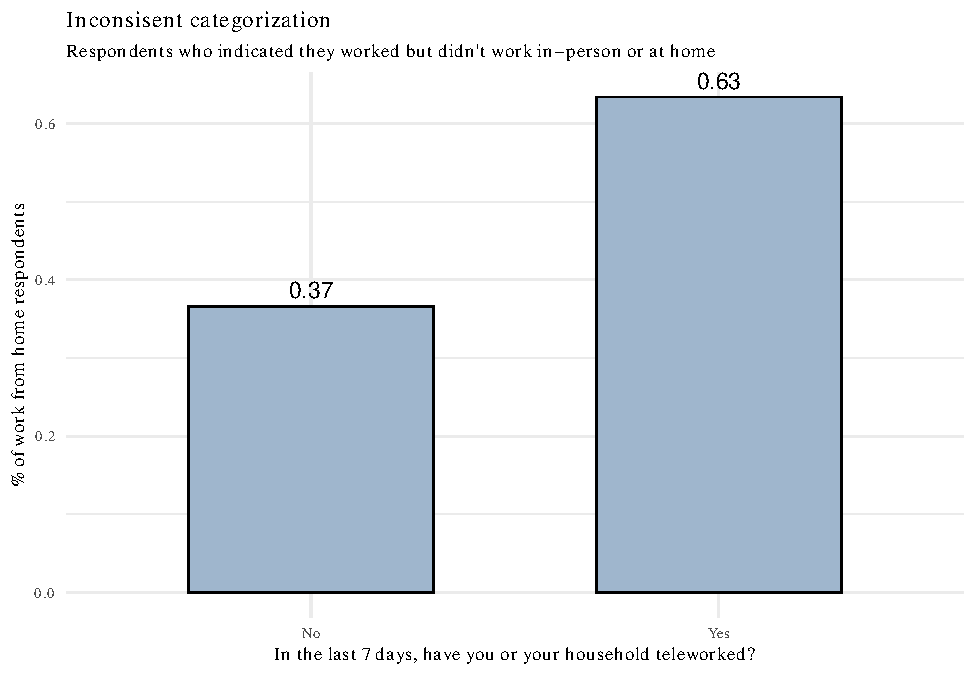
\includegraphics{risk_of_infection_files/figure-latex/unnamed-chunk-12-1.pdf}

\begin{Shaded}
\begin{Highlighting}[]
\FunctionTok{ggsave}\NormalTok{(}\StringTok{"figures/inconsisent\_responses.png"}\NormalTok{)}
\end{Highlighting}
\end{Shaded}

\begin{Shaded}
\begin{Highlighting}[]
\NormalTok{temp\_merge }\OtherTok{\textless{}{-}}\NormalTok{ temp\_merge }\SpecialCharTok{\%\textgreater{}\%} 
\NormalTok{  dplyr}\SpecialCharTok{::}\FunctionTok{mutate}\NormalTok{(}\AttributeTok{setting =} \FunctionTok{as.character}\NormalTok{(setting),}
                \AttributeTok{setting =} \FunctionTok{if\_else}\NormalTok{((setting }\SpecialCharTok{==} \StringTok{"working from home"} \SpecialCharTok{\&}\NormalTok{ teleworked }\SpecialCharTok{==} \DecValTok{2}\NormalTok{),}
                                  \StringTok{"missing"}\NormalTok{,}
\NormalTok{                                  setting)) }\SpecialCharTok{\%\textgreater{}\%}
  \FunctionTok{replace\_with\_na}\NormalTok{(}\AttributeTok{replace =} \FunctionTok{list}\NormalTok{(}\AttributeTok{setting =} \StringTok{"missing"}\NormalTok{))}
\end{Highlighting}
\end{Shaded}

\begin{Shaded}
\begin{Highlighting}[]
\NormalTok{pulse\_grouped }\OtherTok{\textless{}{-}}\NormalTok{ temp\_merge }\SpecialCharTok{\%\textgreater{}\%}
  \FunctionTok{mutate\_if}\NormalTok{(is.character, as.factor)}
\end{Highlighting}
\end{Shaded}

\begin{Shaded}
\begin{Highlighting}[]
\FunctionTok{write.csv}\NormalTok{(pulse\_grouped,}\StringTok{"data\_files/pulse/processed/all\_phases.csv"}\NormalTok{)}
\end{Highlighting}
\end{Shaded}

Using missForest (random forest algorithm implementation) to impute
missing values:

\begin{Shaded}
\begin{Highlighting}[]
\CommentTok{\#imputed \textless{}{-} missForest(pulse\_grouped \%\textgreater{}\% select({-}job))}
\NormalTok{imputed }\OtherTok{\textless{}{-}} \FunctionTok{na.omit}\NormalTok{(pulse\_grouped)}
\end{Highlighting}
\end{Shaded}

\begin{Shaded}
\begin{Highlighting}[]
\NormalTok{pulse\_grouped }\OtherTok{\textless{}{-}} \FunctionTok{read\_csv}\NormalTok{(}\StringTok{"data\_files/pulse/processed/all\_phases.csv"}\NormalTok{)}
\end{Highlighting}
\end{Shaded}

\hypertarget{risk-of-infection-model}{%
\subsubsection{Risk-of-infection model}\label{risk-of-infection-model}}

Having categorized Pulse respondents into their respective work
categories, we now want to create a model to estimate the relative covid
risk for different workers. Because we are ultimately interested in
understanding risk specific to the workplace, we want to distribute
infections between those occurring at work, leisure, or at home. To do
this, we take the following steps:

\textbf{1. Estimate hours in each setting} Under the assumption that
spending more time in a certain setting increases ones probability of
contracting covid in it, we first go about estimating the number of
hours a respondent spends at home, leisure, and the workplace. To do
this, we use pooled state-level ATUS data and determine the average
number of hours respondents in each work status (NILF, unemployed,
employed remote, employed in-person) spend in the three settings.

The first step is to prepare the ATUS data, categorizing respondents
into the work statuses of interest.

Processing ATUS data:

\begin{itemize}
\tightlist
\item
  Respondent file contains information on labor status obtained from
  CPS. We use this to categorize as we do CPS data.

  \begin{itemize}
  \tightlist
  \item
    emp\_status: 1 = Employed, at work. 2 = Employed, absent. 3 =
    Unemployed, on layoff. 4 = Unemployed, looking. 5 = Not in labor
    force.
  \item
    industry: census industry codes
  \item
    occupation: census occupation codes
  \end{itemize}
\end{itemize}

\begin{Shaded}
\begin{Highlighting}[]
\NormalTok{clean\_vars }\OtherTok{\textless{}{-}} \FunctionTok{read.csv}\NormalTok{(}\StringTok{"data\_files/cleanvariables/atus/atus\_cleanvars.csv"}\NormalTok{)}
\NormalTok{cic\_to\_pulse }\OtherTok{\textless{}{-}} \FunctionTok{read.csv}\NormalTok{(}\StringTok{"data\_files/cps\_acs/crosswalk/cic\_to\_pulse.csv"}\NormalTok{)}
\NormalTok{coc\_to\_pulse }\OtherTok{\textless{}{-}} \FunctionTok{read.csv}\NormalTok{(}\StringTok{"data\_files/cps\_acs/crosswalk/coc\_to\_pulse.csv"}\NormalTok{)}
\NormalTok{teleworkable }\OtherTok{\textless{}{-}} \FunctionTok{read.csv}\NormalTok{(}\StringTok{"data\_files/cps\_acs/crosswalk/teleworkable.csv"}\NormalTok{)}
\end{Highlighting}
\end{Shaded}

\begin{Shaded}
\begin{Highlighting}[]
\NormalTok{open }\OtherTok{\textless{}{-}} \ControlFlowTok{function}\NormalTok{(yr,tp)\{}
\NormalTok{  filepath }\OtherTok{=} \FunctionTok{paste0}\NormalTok{(}\StringTok{"data\_files/atus/"}\NormalTok{,yr,}\StringTok{"/atus"}\NormalTok{,tp,}\StringTok{"\_"}\NormalTok{,yr,}\StringTok{".dat"}\NormalTok{)}
\NormalTok{  clean }\OtherTok{\textless{}{-}}\NormalTok{ clean\_vars }\SpecialCharTok{\%\textgreater{}\%} \FunctionTok{filter}\NormalTok{(type }\SpecialCharTok{==}\NormalTok{ tp }\SpecialCharTok{\&}\NormalTok{ year }\SpecialCharTok{==}\NormalTok{ yr)}
\NormalTok{  df }\OtherTok{\textless{}{-}} \FunctionTok{read.delim}\NormalTok{(filepath, }\AttributeTok{header=}\ConstantTok{TRUE}\NormalTok{, }\AttributeTok{sep=}\StringTok{","}\NormalTok{) }\SpecialCharTok{\%\textgreater{}\%}
\NormalTok{    dplyr}\SpecialCharTok{::}\FunctionTok{select}\NormalTok{(clean}\SpecialCharTok{$}\NormalTok{atusname) }\SpecialCharTok{\%\textgreater{}\%}
\NormalTok{    purrr}\SpecialCharTok{::}\FunctionTok{set\_names}\NormalTok{(clean}\SpecialCharTok{$}\NormalTok{newname) }\SpecialCharTok{\%\textgreater{}\%}
    \FunctionTok{mutate}\NormalTok{(}\AttributeTok{year =}\NormalTok{ yr)}
  \FunctionTok{return}\NormalTok{(df)}
\NormalTok{\}}
\end{Highlighting}
\end{Shaded}

\begin{Shaded}
\begin{Highlighting}[]
\NormalTok{atusresp }\OtherTok{\textless{}{-}} \FunctionTok{rbind}\NormalTok{(}\FunctionTok{open}\NormalTok{(}\StringTok{"2020"}\NormalTok{,}\StringTok{"resp"}\NormalTok{),}
                  \FunctionTok{open}\NormalTok{(}\StringTok{"2021"}\NormalTok{,}\StringTok{"resp"}\NormalTok{))}
\end{Highlighting}
\end{Shaded}

We obtain job categories for all ATUS respondents using our CPS
crosswalk which matches Census industries and occupations to one of our
Pulse settings. As we do in the ATUS, we only categorize a respondent as
employed if they've done work for pay or profit in the last 7 days.
Workers who aren't employed are categorized as NILF if their reason for
not working is that they are retired, disabled, or unable to work.

\begin{Shaded}
\begin{Highlighting}[]
\NormalTok{atusresp }\OtherTok{\textless{}{-}}\NormalTok{ atusresp }\SpecialCharTok{\%\textgreater{}\%} 
  \FunctionTok{merge}\NormalTok{(.,cic\_to\_pulse,}\AttributeTok{by=}\StringTok{"industry"}\NormalTok{) }\SpecialCharTok{\%\textgreater{}\%}
  \FunctionTok{merge}\NormalTok{(., coc\_to\_pulse,}\AttributeTok{by=}\FunctionTok{c}\NormalTok{(}\StringTok{"occupation"}\NormalTok{,}\StringTok{"industry"}\NormalTok{,}\StringTok{"industry\_title"}\NormalTok{),}\AttributeTok{all.x=}\ConstantTok{TRUE}\NormalTok{) }\SpecialCharTok{\%\textgreater{}\%}
  \FunctionTok{merge}\NormalTok{(.,teleworkable,}\AttributeTok{by =} \StringTok{"occupation"}\NormalTok{,}\AttributeTok{all.x=}\ConstantTok{TRUE}\NormalTok{) }\SpecialCharTok{\%\textgreater{}\%}
  \FunctionTok{mutate}\NormalTok{(}\AttributeTok{teleworkable =} \FunctionTok{ifelse}\NormalTok{(}\FunctionTok{is.na}\NormalTok{(teleworkable),}\DecValTok{0}\NormalTok{,teleworkable),}
         \AttributeTok{setting =} \FunctionTok{coalesce}\NormalTok{(occupation\_based\_setting,industry\_based\_setting)) }\SpecialCharTok{\%\textgreater{}\%} 
  \FunctionTok{mutate}\NormalTok{(}\AttributeTok{setting =} \FunctionTok{as.character}\NormalTok{(setting),}
         \AttributeTok{casied =} \FunctionTok{as.character}\NormalTok{(caseid)) }\SpecialCharTok{\%\textgreater{}\%}
  \FunctionTok{mutate}\NormalTok{(}\AttributeTok{setting =} \FunctionTok{ifelse}\NormalTok{(any\_work }\SpecialCharTok{==} \DecValTok{2}\NormalTok{,}\StringTok{"Unemployed"}\NormalTok{,}
                          \FunctionTok{ifelse}\NormalTok{(any\_work }\SpecialCharTok{\%in\%} \FunctionTok{c}\NormalTok{(}\DecValTok{3}\NormalTok{,}\DecValTok{4}\NormalTok{,}\DecValTok{5}\NormalTok{),}\StringTok{"NILF"}\NormalTok{,setting)))}
\end{Highlighting}
\end{Shaded}

Now we get atus-cps file which contains information on the state and
education level of respondents.

\begin{Shaded}
\begin{Highlighting}[]
\CommentTok{\#Convert fips codes into state names}
\NormalTok{fips }\OtherTok{\textless{}{-}} \FunctionTok{unique}\NormalTok{(}\FunctionTok{get}\NormalTok{(}\FunctionTok{data}\NormalTok{(}\StringTok{"fips\_codes"}\NormalTok{)) }\SpecialCharTok{\%\textgreater{}\%} 
              \FunctionTok{select}\NormalTok{(state\_code,state\_name) }\SpecialCharTok{\%\textgreater{}\%} 
\NormalTok{              dplyr}\SpecialCharTok{::}\FunctionTok{rename}\NormalTok{(}\StringTok{"state"} \OtherTok{=} \StringTok{"state\_code"}\NormalTok{) }\SpecialCharTok{\%\textgreater{}\%}
              \FunctionTok{mutate}\NormalTok{(}\AttributeTok{state =} \FunctionTok{as.numeric}\NormalTok{(state)))}
\end{Highlighting}
\end{Shaded}

\begin{Shaded}
\begin{Highlighting}[]
\NormalTok{atuscps }\OtherTok{\textless{}{-}} \FunctionTok{rbind}\NormalTok{(}\FunctionTok{open}\NormalTok{(}\StringTok{"2020"}\NormalTok{,}\StringTok{"cps"}\NormalTok{),}
                 \FunctionTok{open}\NormalTok{(}\StringTok{"2021"}\NormalTok{,}\StringTok{"cps"}\NormalTok{))}
\end{Highlighting}
\end{Shaded}

\begin{Shaded}
\begin{Highlighting}[]
\CommentTok{\# Education variable into our four categories}
\NormalTok{atuscps }\OtherTok{\textless{}{-}}\NormalTok{ atuscps }\SpecialCharTok{\%\textgreater{}\%}
  \CommentTok{\# File contains responses for household members as well. We filter for atus\_respondent = 1, corresponding to person interviewed for ATUS}
  \FunctionTok{filter}\NormalTok{(atus\_respondent }\SpecialCharTok{==} \DecValTok{1}\NormalTok{) }\SpecialCharTok{\%\textgreater{}\%}
  \FunctionTok{merge}\NormalTok{(.,fips,}\AttributeTok{by=}\StringTok{"state"}\NormalTok{) }\SpecialCharTok{\%\textgreater{}\%}
  \FunctionTok{mutate}\NormalTok{(}\AttributeTok{state =}\NormalTok{ state\_name) }\SpecialCharTok{\%\textgreater{}\%}
  \FunctionTok{select}\NormalTok{(}\SpecialCharTok{{-}}\NormalTok{state\_name) }\SpecialCharTok{\%\textgreater{}\%}
  \FunctionTok{mutate}\NormalTok{(}\AttributeTok{caseid =} \FunctionTok{as.character}\NormalTok{(caseid)) }\SpecialCharTok{\%\textgreater{}\%}
  \FunctionTok{mutate}\NormalTok{(}\AttributeTok{education =} \FunctionTok{case\_when}\NormalTok{(}
\NormalTok{    education }\SpecialCharTok{\textless{}=} \DecValTok{38} \SpecialCharTok{\textasciitilde{}} \StringTok{"Less than HS graduate"}\NormalTok{,}
\NormalTok{    education }\SpecialCharTok{==} \DecValTok{39} \SpecialCharTok{\textasciitilde{}} \StringTok{"HS graduate or GED"}\NormalTok{,}
\NormalTok{    education }\SpecialCharTok{\textgreater{}} \DecValTok{39} \SpecialCharTok{\&}\NormalTok{ education }\SpecialCharTok{\textless{}=} \DecValTok{42} \SpecialCharTok{\textasciitilde{}} \StringTok{"Some college or associate\textquotesingle{}s degree"}\NormalTok{,}
\NormalTok{    education }\SpecialCharTok{\textgreater{}} \DecValTok{42} \SpecialCharTok{\&}\NormalTok{ education }\SpecialCharTok{\textless{}=} \DecValTok{46} \SpecialCharTok{\textasciitilde{}} \StringTok{"Bachelor\textquotesingle{}s degree or higher"}
\NormalTok{  ))}
\end{Highlighting}
\end{Shaded}

\begin{Shaded}
\begin{Highlighting}[]
\CommentTok{\#Merge with respondent file for a complete view:}
\NormalTok{atusresp }\OtherTok{\textless{}{-}} \FunctionTok{merge}\NormalTok{(atusresp }\SpecialCharTok{\%\textgreater{}\%} \FunctionTok{mutate}\NormalTok{(}\AttributeTok{caseid =} \FunctionTok{as.character}\NormalTok{(caseid)),}
\NormalTok{                  atuscps }\SpecialCharTok{\%\textgreater{}\%} \FunctionTok{mutate}\NormalTok{(}\AttributeTok{caseid =} \FunctionTok{as.character}\NormalTok{(caseid)),}
                  \AttributeTok{by=}\FunctionTok{c}\NormalTok{(}\StringTok{"caseid"}\NormalTok{,}\StringTok{"year"}\NormalTok{))}
\end{Highlighting}
\end{Shaded}

Finally, we can merge with activity data to get time distribution across
settings. ATUS activity file includes activity-level information
collected in ATUS, including activity code, location, duration, activity
start and stop times.

\begin{Shaded}
\begin{Highlighting}[]
\CommentTok{\#Note, two different variables available for the cumulative duration of an activity. In the one we use, the last activity is truncated at 4 am.}
\NormalTok{atusact }\OtherTok{\textless{}{-}} \FunctionTok{rbind}\NormalTok{(}\FunctionTok{open}\NormalTok{(}\StringTok{"2020"}\NormalTok{,}\StringTok{"act"}\NormalTok{),}
                 \FunctionTok{open}\NormalTok{(}\StringTok{"2021"}\NormalTok{,}\StringTok{"act"}\NormalTok{))}
\end{Highlighting}
\end{Shaded}

Location is not collected for activities with activity codes of 0101xx
(sleeping), 0102xx (grooming), 0104xx (personal activites), 500105 (none
of your business), or 500106 (gap can't remember). We assume sleeping,
grooming, and personal activities occured in the household. Finally, we
remove location code 89, ``Unspecified place''.

\begin{Shaded}
\begin{Highlighting}[]
\NormalTok{atusact }\OtherTok{\textless{}{-}}\NormalTok{ atusact }\SpecialCharTok{\%\textgreater{}\%}
  \FunctionTok{mutate}\NormalTok{(}\AttributeTok{location =} \FunctionTok{ifelse}\NormalTok{(tier1code }\SpecialCharTok{==} \DecValTok{1} \SpecialCharTok{\&}\NormalTok{ tier2code }\SpecialCharTok{\%in\%} \FunctionTok{c}\NormalTok{(}\DecValTok{1}\NormalTok{,}\DecValTok{2}\NormalTok{,}\DecValTok{3}\NormalTok{),}\DecValTok{1}\NormalTok{,location)) }\SpecialCharTok{\%\textgreater{}\%}
  \FunctionTok{filter}\NormalTok{(location }\SpecialCharTok{!=} \SpecialCharTok{{-}}\DecValTok{1} \SpecialCharTok{\&}\NormalTok{ location }\SpecialCharTok{!=} \DecValTok{89}\NormalTok{) }\SpecialCharTok{\%\textgreater{}\%}
  \FunctionTok{mutate}\NormalTok{(}\AttributeTok{caseid =} \FunctionTok{as.character}\NormalTok{(caseid)) }\SpecialCharTok{\%\textgreater{}\%}
  \FunctionTok{merge}\NormalTok{(.,atusresp,}\AttributeTok{by=}\FunctionTok{c}\NormalTok{(}\StringTok{"caseid"}\NormalTok{,}\StringTok{"year"}\NormalTok{))}
\end{Highlighting}
\end{Shaded}

\textbf{Categorizing in-person and remote workers}

Currently, we categorize workers based on their industry and occupation,
but do not specify whether they are remote or in-person. The CPS added a
question on whether the respondent did any teleworking:

\emph{"At any time in the LAST 4 WEEKS, did (you/name) telework or work
at home for pay BECAUSE OF THE CORONAVIRUS PANDEMIC?}

However, this captures a different set of people than the Pulse, which
asks:

\emph{``Since January 1, 2021 {[}or ``In the last 7 days'' for later
surveys{]}, have you worked or volunteered outside your home?''}

Three main differences with the question:

\begin{enumerate}
\def\labelenumi{\arabic{enumi}.}
\tightlist
\item
  In the Pulse, we categorize anyone who worked outside the home at any
  point as in-person. In the CPS, anyone who worked remotely is remote.
  E.g., If person X worked 3 days at home and 2 days in-person because
  of covid policied, they'd be remote in the CPS but in-person in the
  Pulse.
\item
  The timeframe for the CPS is the last 4 weeks while the Pulse asks
  about the last 7 days (for most phases)
\item
  The CPS only captures those who teleworked \emph{because} of covid.
\end{enumerate}

Because of all the discrepancies, using data from the ATUS itself could
be a better stratey to replicate the Pulse question. As a first step we:

\begin{itemize}
\tightlist
\item
  Get all respondents who did work in the last 7 days (i.e., those we
  label as ``employed'' in the Pulse)
\item
  From the hours these respondents spent working, calculate how many
  were at home and outside the home
\item
  If a respondent spent any time working outside the home, they are
  categorized as in-person. This captures the ``low bar'' to in-person
  working set by the Pulse.
\item
  If a respondent spent all work hours inside the home, they are
  categorized as remote.
\end{itemize}

An issue with this strategy is that some respondents did no work on the
day they were surveyed (were surveyed on the weekend, etc). For cases
where we have no ATUS information, we move on the next ``best'' data,
the CPS question asking if they were remotely. Those who said they
teleworked are categorized as remote, those that didn't are in-person.

Finally, due to the non-response rate to the teleworking question on the
CPS, as a last resort, we use the Dingel and Neiman categorizations to
know if the respondent's job is teleworkable or not.

\begin{Shaded}
\begin{Highlighting}[]
\NormalTok{cats }\OtherTok{\textless{}{-}}\NormalTok{ atusact }\SpecialCharTok{\%\textgreater{}\%}
  \FunctionTok{filter}\NormalTok{(tier1code }\SpecialCharTok{==} \DecValTok{5}\NormalTok{) }\SpecialCharTok{\%\textgreater{}\%}
\NormalTok{  dplyr}\SpecialCharTok{::}\FunctionTok{mutate}\NormalTok{(}\AttributeTok{top\_location =} \FunctionTok{ifelse}\NormalTok{(location }\SpecialCharTok{==} \DecValTok{1}\NormalTok{,}\StringTok{"Home"}\NormalTok{,}\StringTok{"Other"}\NormalTok{)) }\SpecialCharTok{\%\textgreater{}\%}
\NormalTok{  dplyr}\SpecialCharTok{::}\FunctionTok{group\_by}\NormalTok{(caseid,top\_location) }\SpecialCharTok{\%\textgreater{}\%}
\NormalTok{  dplyr}\SpecialCharTok{::}\FunctionTok{summarize}\NormalTok{(}\AttributeTok{work\_time =} \FunctionTok{sum}\NormalTok{(duration)) }\SpecialCharTok{\%\textgreater{}\%}
\NormalTok{  dplyr}\SpecialCharTok{::}\FunctionTok{mutate}\NormalTok{(}\AttributeTok{work\_time =}\NormalTok{ work\_time}\SpecialCharTok{/}\FunctionTok{sum}\NormalTok{(work\_time)) }\SpecialCharTok{\%\textgreater{}\%}
  \FunctionTok{spread}\NormalTok{(top\_location,work\_time) }\SpecialCharTok{\%\textgreater{}\%}
  \FunctionTok{replace}\NormalTok{(}\FunctionTok{is.na}\NormalTok{(.),}\DecValTok{0}\NormalTok{) }\SpecialCharTok{\%\textgreater{}\%}
  \FunctionTok{mutate}\NormalTok{(}\AttributeTok{inperson =} \FunctionTok{ifelse}\NormalTok{(Other }\SpecialCharTok{\textgreater{}} \DecValTok{0}\NormalTok{,}\DecValTok{1}\NormalTok{,}\DecValTok{0}\NormalTok{))}
\NormalTok{atusact }\OtherTok{\textless{}{-}}\NormalTok{ atusact }\SpecialCharTok{\%\textgreater{}\%} 
  \FunctionTok{mutate}\NormalTok{(}\AttributeTok{top\_category =} \FunctionTok{case\_when}\NormalTok{(}
\NormalTok{    setting }\SpecialCharTok{==} \StringTok{"NILF"} \SpecialCharTok{\textasciitilde{}} \StringTok{"NILF"}\NormalTok{,}
\NormalTok{    setting }\SpecialCharTok{==} \StringTok{"Unemployed"} \SpecialCharTok{\textasciitilde{}} \StringTok{"Unemployed"}\NormalTok{,}
\NormalTok{    caseid }\SpecialCharTok{\%in\%}\NormalTok{ cats[cats}\SpecialCharTok{$}\NormalTok{inperson }\SpecialCharTok{==} \DecValTok{1}\NormalTok{,]}\SpecialCharTok{$}\NormalTok{caseid }\SpecialCharTok{\textasciitilde{}} \StringTok{"In{-}person"}\NormalTok{,}
\NormalTok{    caseid }\SpecialCharTok{\%in\%}\NormalTok{ cats[cats}\SpecialCharTok{$}\NormalTok{inperson }\SpecialCharTok{==} \DecValTok{0}\NormalTok{ ,]}\SpecialCharTok{$}\NormalTok{caseid }\SpecialCharTok{\textasciitilde{}} \StringTok{"Remote"}\NormalTok{,}
\NormalTok{    work\_at\_home }\SpecialCharTok{==} \DecValTok{1} \SpecialCharTok{\textasciitilde{}} \StringTok{"Remote"}\NormalTok{,}
\NormalTok{    work\_at\_home }\SpecialCharTok{==} \DecValTok{2} \SpecialCharTok{\textasciitilde{}} \StringTok{"In{-}person"}\NormalTok{,}
\NormalTok{    teleworkable }\SpecialCharTok{==} \DecValTok{0} \SpecialCharTok{\textasciitilde{}} \StringTok{"In{-}person"}\NormalTok{,}
\NormalTok{    teleworkable }\SpecialCharTok{==} \DecValTok{1} \SpecialCharTok{\textasciitilde{}} \StringTok{"Remote"}
\NormalTok{  ))}
\end{Highlighting}
\end{Shaded}

To assess our crosswalk, we can compare the estimated population of
remote workers from the Pulse and the ATUS.

First, we can convert Pulse weeks into months:

Week 34: July 21 - August 2 (July) Week 35: August 4 - August 16 (100\%
August) Week 36: August 18 - August 30 (100\% August) Week 37: September
1 - September 13 (100\% September) Week 38: September 15 - September 27
(100\% September) Week 39: September 29 - October 11 (October)

Just comparing phase 3.2 and onward:

\begin{Shaded}
\begin{Highlighting}[]
\NormalTok{wfh\_est }\OtherTok{\textless{}{-}}\NormalTok{ pulse\_grouped }\SpecialCharTok{\%\textgreater{}\%}
  \FunctionTok{mutate}\NormalTok{(}\AttributeTok{month =} \FunctionTok{case\_when}\NormalTok{(}
\NormalTok{    week }\SpecialCharTok{==} \DecValTok{28} \SpecialCharTok{\textasciitilde{}} \DecValTok{4}\NormalTok{,}
\NormalTok{    week }\SpecialCharTok{==} \DecValTok{29} \SpecialCharTok{\textasciitilde{}} \DecValTok{5}\NormalTok{,}
\NormalTok{    week }\SpecialCharTok{==} \DecValTok{30} \SpecialCharTok{\textasciitilde{}} \DecValTok{5}\NormalTok{,}
\NormalTok{    week }\SpecialCharTok{==} \DecValTok{31} \SpecialCharTok{\textasciitilde{}} \DecValTok{5}\NormalTok{,}
\NormalTok{    week }\SpecialCharTok{==} \DecValTok{32} \SpecialCharTok{\textasciitilde{}} \DecValTok{6}\NormalTok{,}
\NormalTok{    week }\SpecialCharTok{==} \DecValTok{33} \SpecialCharTok{\textasciitilde{}} \DecValTok{6}\NormalTok{,}
\NormalTok{    week }\SpecialCharTok{==} \DecValTok{34} \SpecialCharTok{\textasciitilde{}} \DecValTok{7}\NormalTok{,}
\NormalTok{    week }\SpecialCharTok{==} \DecValTok{35} \SpecialCharTok{\textasciitilde{}} \DecValTok{8}\NormalTok{,}
\NormalTok{    week }\SpecialCharTok{==} \DecValTok{36} \SpecialCharTok{\textasciitilde{}} \DecValTok{8}\NormalTok{,}
\NormalTok{    week }\SpecialCharTok{==} \DecValTok{37} \SpecialCharTok{\textasciitilde{}} \DecValTok{9}\NormalTok{,}
\NormalTok{    week }\SpecialCharTok{==} \DecValTok{38} \SpecialCharTok{\textasciitilde{}} \DecValTok{9}\NormalTok{,}
\NormalTok{    week }\SpecialCharTok{==} \DecValTok{39} \SpecialCharTok{\textasciitilde{}} \DecValTok{10}\NormalTok{,}
\NormalTok{    week }\SpecialCharTok{==} \DecValTok{40} \SpecialCharTok{\textasciitilde{}} \DecValTok{12}
\NormalTok{  )) }\SpecialCharTok{\%\textgreater{}\%}
  \FunctionTok{na.omit}\NormalTok{() }\SpecialCharTok{\%\textgreater{}\%}
  \FunctionTok{filter}\NormalTok{(}\SpecialCharTok{!}\NormalTok{(job }\SpecialCharTok{\%in\%} \FunctionTok{c}\NormalTok{(}\StringTok{"Unemployed"}\NormalTok{,}\StringTok{"NILF"}\NormalTok{))) }\SpecialCharTok{\%\textgreater{}\%}
\NormalTok{  dplyr}\SpecialCharTok{::}\FunctionTok{group\_by}\NormalTok{(month,week,setting) }\SpecialCharTok{\%\textgreater{}\%}
\NormalTok{  dplyr}\SpecialCharTok{::}\FunctionTok{summarise}\NormalTok{(}\AttributeTok{total =} \FunctionTok{sum}\NormalTok{(weight)) }\SpecialCharTok{\%\textgreater{}\%}
\NormalTok{  dplyr}\SpecialCharTok{::}\FunctionTok{mutate}\NormalTok{(}\AttributeTok{percent =}\NormalTok{ total}\SpecialCharTok{/}\FunctionTok{sum}\NormalTok{(total)) }\SpecialCharTok{\%\textgreater{}\%}
\NormalTok{  dplyr}\SpecialCharTok{::}\FunctionTok{group\_by}\NormalTok{(month,setting) }\SpecialCharTok{\%\textgreater{}\%}
\NormalTok{  dplyr}\SpecialCharTok{::}\FunctionTok{summarise}\NormalTok{(}\AttributeTok{percent =} \FunctionTok{mean}\NormalTok{(percent)) }\SpecialCharTok{\%\textgreater{}\%}
  \FunctionTok{filter}\NormalTok{(setting }\SpecialCharTok{==} \StringTok{"working from home"}\NormalTok{) }\SpecialCharTok{\%\textgreater{}\%}
  \FunctionTok{select}\NormalTok{(percent) }\SpecialCharTok{\%\textgreater{}\%}
  \FunctionTok{mutate}\NormalTok{(}\AttributeTok{type =} \StringTok{"Pulse"}\NormalTok{)}
\end{Highlighting}
\end{Shaded}

\begin{Shaded}
\begin{Highlighting}[]
\NormalTok{wfh\_est }\OtherTok{\textless{}{-}} \FunctionTok{rbind}\NormalTok{(wfh\_est,atusact }\SpecialCharTok{\%\textgreater{}\%}
  \FunctionTok{filter}\NormalTok{(month }\SpecialCharTok{\%in\%} \FunctionTok{c}\NormalTok{(}\DecValTok{4}\NormalTok{,}\DecValTok{5}\NormalTok{,}\DecValTok{6}\NormalTok{,}\DecValTok{7}\NormalTok{,}\DecValTok{8}\NormalTok{,}\DecValTok{9}\NormalTok{,}\DecValTok{10}\NormalTok{,}\DecValTok{12}\NormalTok{) }\SpecialCharTok{\&}\NormalTok{ year }\SpecialCharTok{==} \DecValTok{2021} \SpecialCharTok{\&}\NormalTok{ top\_category }\SpecialCharTok{\%in\%} \FunctionTok{c}\NormalTok{(}\StringTok{"In{-}person"}\NormalTok{,}\StringTok{"Remote"}\NormalTok{)) }\SpecialCharTok{\%\textgreater{}\%}
\NormalTok{  dplyr}\SpecialCharTok{::}\FunctionTok{group\_by}\NormalTok{(month,top\_category) }\SpecialCharTok{\%\textgreater{}\%}
\NormalTok{  dplyr}\SpecialCharTok{::}\FunctionTok{summarise}\NormalTok{(}\AttributeTok{total =} \FunctionTok{sum}\NormalTok{(weight)) }\SpecialCharTok{\%\textgreater{}\%}
\NormalTok{  dplyr}\SpecialCharTok{::}\FunctionTok{mutate}\NormalTok{(}\AttributeTok{percent =}\NormalTok{ total}\SpecialCharTok{/}\FunctionTok{sum}\NormalTok{(total)) }\SpecialCharTok{\%\textgreater{}\%}
  \FunctionTok{filter}\NormalTok{(top\_category }\SpecialCharTok{==} \StringTok{"Remote"}\NormalTok{) }\SpecialCharTok{\%\textgreater{}\%}
  \FunctionTok{select}\NormalTok{(percent) }\SpecialCharTok{\%\textgreater{}\%}
  \FunctionTok{mutate}\NormalTok{(}\AttributeTok{type =} \StringTok{"ATUS"}\NormalTok{))}
\end{Highlighting}
\end{Shaded}

\begin{Shaded}
\begin{Highlighting}[]
\NormalTok{wfh\_est }\SpecialCharTok{\%\textgreater{}\%}
  \FunctionTok{spread}\NormalTok{(type,percent) }\SpecialCharTok{\%\textgreater{}\%}
  \FunctionTok{kable}\NormalTok{()}
\end{Highlighting}
\end{Shaded}

\begin{tabular}{r|r|r}
\hline
month & ATUS & Pulse\\
\hline
4 & 0.2800395 & NA\\
\hline
5 & 0.2692919 & NA\\
\hline
6 & 0.2456256 & NA\\
\hline
7 & 0.2595613 & 0.3139100\\
\hline
8 & 0.2682624 & 0.3218231\\
\hline
9 & 0.2403164 & 0.3163837\\
\hline
10 & 0.1955976 & 0.2957413\\
\hline
12 & 0.1935417 & 0.3027447\\
\hline
\end{tabular}

\begin{Shaded}
\begin{Highlighting}[]
\NormalTok{wfh\_est }\SpecialCharTok{\%\textgreater{}\%}
  \FunctionTok{ggplot}\NormalTok{(}\FunctionTok{aes}\NormalTok{(}\AttributeTok{x=}\NormalTok{month,}\AttributeTok{y=}\NormalTok{percent,}\AttributeTok{color=}\NormalTok{type)) }\SpecialCharTok{+} 
  \FunctionTok{geom\_point}\NormalTok{() }\SpecialCharTok{+} 
  \FunctionTok{geom\_line}\NormalTok{() }\SpecialCharTok{+} 
  \FunctionTok{theme\_bw}\NormalTok{() }\SpecialCharTok{+} 
  \FunctionTok{labs}\NormalTok{(}\AttributeTok{x=}\StringTok{"Month"}\NormalTok{,}\AttributeTok{y=}\StringTok{"\% labor force"}\NormalTok{,}\AttributeTok{title =} \StringTok{"Remote employee estimate {-} ATUS vs. Pulse"}\NormalTok{) }\SpecialCharTok{+} 
  \FunctionTok{theme}\NormalTok{(}\AttributeTok{text =} \FunctionTok{element\_text}\NormalTok{(}\AttributeTok{family =} \StringTok{"Georgia"}\NormalTok{,}\AttributeTok{size=}\DecValTok{11}\NormalTok{)) }\SpecialCharTok{+} 
  \FunctionTok{scale\_color\_discrete}\NormalTok{(}\AttributeTok{name =} \StringTok{"Focus of chapter"}\NormalTok{) }\SpecialCharTok{+}
  \FunctionTok{scale\_color\_manual}\NormalTok{(}\AttributeTok{values=}\FunctionTok{wes\_palette}\NormalTok{(}\AttributeTok{n=}\DecValTok{2}\NormalTok{, }\AttributeTok{name=}\StringTok{"Chevalier1"}\NormalTok{,}\AttributeTok{type=}\StringTok{"continuous"}\NormalTok{))}
\end{Highlighting}
\end{Shaded}

\includegraphics{risk_of_infection_files/figure-latex/unnamed-chunk-33-1.pdf}

Because we are averaging time in each setting from across the pandemic
period, we risk over or underestimating the number of infections
occuring in a given setting. If, for example, the time spent during
leisure increased significantly in the last two months we study, our
leisure hour average will underestimate leisure time in those two months
and result in an underestimate of infections. The upshot: for our
procedure to be accurate, we would want the percent of time spent in
each setting to remain consistent. With this in mind, we looked at ATUS
data from April 2020 to December 2021 to look at time spent in each
setting per month:

\end{document}
